\documentclass[ 12pt]{article}
%\documentclass[ 12pt]{book}

\usepackage{times,vmargin,url,html}
\setmarginsrb{3cm}{1cm}{2cm}{1cm}{1cm}{1cm}{1cm}{1cm}
%\setpapersize{A4}
\usepackage{dr-bibbib} %-sort-year}

\usepackage{color,time,array}
\pagecolor{yellow}
%\pagecolor{cyan}
\pagecolor{white}

\newcommand{\keywords}[1]{\textbf{Keywords:} #1} %\\ \clearpage %\tableofcontents\clearpage}
%

\usepackage{xcolor}
%\usepackage{b2latex}

%\IEEEoverridecommandlockouts
% The preceding line is only needed to identify funding in the first footnote. If that is unneeded, please comment it out.
\usepackage{cite,time}
\usepackage{amsmath,amssymb,amsfonts}
\usepackage{algorithmic}
\usepackage{graphicx}
\usepackage{textcomp}
\usepackage{xcolor,time,url,nbcode,version}
\usepackage{wrapfig}
%\usepackage{b2latex}
\usepackage{caption}
\usepackage{bm}
\usepackage{float}
\usepackage{enumitem}
\usepackage{listings}
\usepackage{bussproofs}
\usepackage{wrapfig,setspace}
%\usepackage{lstcoq}
\usepackage{xspace}
\usepackage{hyperref}

\def\BibTeX{{\rm B\kern-.05em{\sc i\kern-.025em b}\kern-.08em
    T\kern-.1667em\lower.7ex\hbox{E}\kern-.125emX}}
\pagestyle{plain}
\pagenumbering{arabic}
\let\proof\relax
\let\endproof\relax
\let\example\relax
\let\endexample\relax



\usepackage{mathpartir}
\usepackage{amssymb,amsmath,amsthm}
\usepackage{rotating}
\usepackage{blox}
\usepackage{graphicx} 
\usepackage{eventblst}
\usepackage{cite}
\usepackage{dafny}
 

% \usepackage{amssymb,amsmath} problematic with acm, use \usepackage{newtxtext,newtxmath}
% \usepackage{newtxtext,newtxmath}



%%%%%%%%%%%%%%%%%%%%%%%%%%%%%%%%%%%%%%%%%%%%%%%%%%%%%%%%%%%%%%%%%%%%%%%%
% Macros for proof-reading
%%%%%%%%%%%%%%%%%%%%%%%%%%%%%%%%%%%%%%%%%%%%%%%%%%%%%%%%%%%%%%%%%%%%%%%%


\usepackage{xcolor}
\usepackage{ifthen}
\newboolean{showcomments}
\setboolean{showcomments}{true} % toggle to show or hide comments

\ifthenelse{\boolean{showcomments}} { 
    \usepackage{outlines}
    \let\oldoutline\outline
    \def\outline{\oldoutline\color{blue}}

    \usepackage[normalem]{ulem}
    \def \ifempty#1{\def\temp{#1} \ifx\temp\empty }
    \newcommand{\xnote}[3][]{\textcolor{red}{#2}$\rightarrow$ \textcolor{blue}{\textbf{#1} #3}}
    \newcommand{\xtodo}[2][]{\xnote[#1]{}{#2}}

    \newcommand{\xreplace}[3][]{\ifempty {#3} \textcolor{red}{\textbf{#1} \sout{#2}} \else \textcolor{red}{\sout{#2}} $\rightarrow$ \textcolor{blue}{\textbf{#1} "#3"} \fi}
    \newcommand{\xdelete}[2][]{\xreplace[#1]{#2}{}}
    \newcommand{\xadd}[2][]{\xreplace[#1]{}{#2}}
} {
    \newcommand{\xnote}[3][]{}
    \newcommand{\xtodo}[2][]{}
    \newcommand{\xreplace}[3][]{#3}
    \newcommand{\xdelete}[2][]{}
    \newcommand{\xadd}[2][]{#2}
    \def\outline{}
    \def\1{}
    \def\2{}
    \def\3{}
    \def\4{}
}
% % % % % % % % % % % % % % % % % % % % % % % % %

\newcommand{\dnote}[2]{\xnote[DM]{#1}{#2}}
\newcommand{\dtodo}[1]{\xtodo[DM]{#1}}
\newcommand{\dreplace}[2]{\xreplace[DM]{#1}{#2}}
\newcommand{\ddelete}[1]{\xdelete[DM]{#1}}
\newcommand{\dadd}[1]{\xadd[DM]{#1}}


\newcommand{\znote}[2]{\xnote[ZC]{#1}{#2}}
\newcommand{\ztodo}[1]{\xtodo[ZC]{#1}}
\newcommand{\zreplace}[2]{\xreplace[ZC]{#1}{#2}}
\newcommand{\zdelete}[1]{\xdelete[ZC]{#1}}
\newcommand{\zadd}[1]{\xadd[ZC]{#1}}

% % % % % % % % % % % % % % % % % % % % % % % % %

\newcommand{\PB}{{\sc\bf  PB}\;}
\newcommand{\MO}{{\sc\bf  MO}\;}
\newcommand{\GC}{{\sc\bf  GC}\;}
\newcommand{\HP}{{\sc\bf  HP}\;}
\newcommand{\dL}{d${\cal  L}$\;}

\newcommand*\choice[0]{[\!]}
\newcommand{\set}[1]{\{#1\}}
\newcommand{\aloop}[1]{\textbf{do}\  #1  \ \textbf{od}}

\makeatletter
\def\footnoterule{\relax%
  \kern-5pt
  \hbox to \columnwidth{\hfill\vrule width 0.9\columnwidth height 0.4pt\hfill}
  \kern4.6pt}
\makeatother
%ddd -aal\renewcommand{\baselinestretch}{0.90}
\newtheorem{myexample}{Example}[section]
\newtheorem{mytheorem}{Property}
%\newtheorem{definition}{Definition}
%\includeversion{check}
% \excludeversion{check}
% \excludeversion{long}
%%%%%%%%%%%%%%%%%%%%%%%%%%%%%%%%%%%%%%%%%%%%%%%%
%%%%%%%%%%%%%%%%%%%%%%%%%%%%%%%%%%%%%%%%%%%%%%%%
\newtheorem{exemple}{Example}
%\newtheorem{theorem}{Theorem}
%\newcommand{\white}[1]{\textcolor{white}{#1}}

%\newtheorem{comm}{Teaching Point}
%\newenvironment{comm}{\iffalse}{\fi}
%\excludeversion{comm}

\input eb2latex

\pagestyle{plain}
%%%%%%%%%%%%%%%%%%%%%%%%%%%%%%%%%%%%%%%%%%%%%%%%
%%%%%%%%%%%%%%%%%%%%%%%%%%%%%%%%%%%%%%%%%%%%%%%%
\title{Dominique Méry's Home Page}
\author{Dominique M\'ery\\
LORIA \& Telecom Nancy\\ Universit\'e de Lorraine\\
\url{https://members.loria.fr/Mery}\\ \url{dominique-dot-mery-at-loria-fr}}

\date{\today}

\begin{document}
\newcounter{ex}  \setcounter{ex}{1}
\maketitle





\noindent
\begin{tabular}{m{0.5\textwidth} m{0.5\textwidth}}
  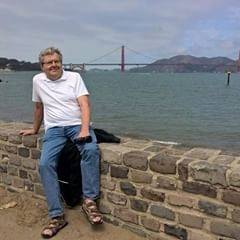
\includegraphics{./images/merysf.jpg}  &
                                           \begin{minipage}{0.5\linewidth}
                                             Dominique Méry is  professor of computing science at  \href{https://www.univ-lorraine.fr}{Université  de 
Lorraine}, where he teaches     formal methods and related topics    in the school of computer engineering 
\href{https://telecomnancy.univ-lorraine.fr}{Telecom Nancy} and in the Faculty of Science and Technology.  His 
research activities are developed in the laboratory  \href{https://www.loria.fr}{LORIA} joint 
structure  of CNRS, INRIA and  Université de Lorraine.  You can 
contact him  using the email of LORIA.
\end{minipage}
\end{tabular}


\iffalse
\begin{minipage}{1.0\linewidth}
\begin{minipage}{0.5\linewidth}

  % \href{https://mery54.github.io/mery/images/merysf.jpg}{images/merysf.jpg}
   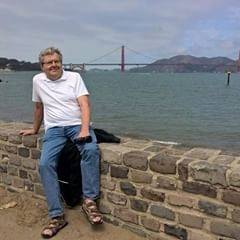
\includegraphics{./images/merysf.jpg}
  
\end{minipage}\ \hfill \  \begin{minipage}{0.4\linewidth}
Dominique Méry is  professor of Computing Science at  \href{https://www.univ-lorraine.fr}{Université  de 
Lorraine}, where he teaches     formal methods and related topics    in the school of computer engineering 
Telecom Nancy and in the Faculty of Science and Technology.  His 
research activities are developed in the laboratory  \href{https://ww.loria.fr}{LORIA} joint 
structure  of CNRS, INRIA and  Université de Lorraine.  You can 
contact him  using the email of LORIA.
  
\end{minipage}
  
\end{minipage}
\fi



\tableofcontents

\section{Teaching}





\begin{itemize}

\item[] \href{https://mery54.github.io/teaching/mosos/}{Lectures MOSOS 
    on formal modelling}.


  \item[] \href{https://mery54.github.io/teaching/mvsi/}{Lectures MVSI 
    on  verification  nd modelling of programs}.


  
\end{itemize}

\section{Research}


\subsection{Current scientific activities}


  My current  scientific activities focus  on proof-based developement
  of distributed  algorithms  using    the refinement, as     well as
  modelling and certification of medical devices.

  First, distributed  algorithms,  recently redeveloped by refinement,
  are population protocols  which  are  leading  to extension  of  the
  refinement,  and self-$\star$ algorithms. The  main difficulty is to
  deal    with liveness   and   fairness properties,  when  considering
  population protocols for  instance, and with explicit assumptions as for instance 
  oracles for faults.

  Second,   medical  devices  lead  to propose a  refinement-based methodology
  applicable  for   certification    of  cyber-physical  systems   and
  human-in-the-loop  systems.  Two   collaborations (NASA Ames and  CHU
  Nancy) are interacting with us for these topics.



Finally, the IMPEX (http://impex.loria.fr) project leads me to deal with the integration of
the explicit semantics in  proof-based development of software
systems. Recently, I have obtained two new projects ANR FORMEDICIS
(2017-2022) on verification of HMI, extending IMPEX, and ANR project
DISCONT (http://discont.loria.fr)  on hybrid models and  refinement.







\section{Curriculum Vitae}
\newcommand{\nancyIesial}{\ca{Universit\'{e} de Nancy I~:~Ecole sup\'{e}rieure d'informatique appliqu\'{e}e de Lorraine}}
\newcommand{\inancyIesial}{Universit\'{e} Henri Poincar\'e -  Nancy I}
%\newcommand{\esial}{Ecole sup\'{e}rieure d'informatique appliqu\'{e}e de Lorraine}
\newcommand{\nancyIesstin}{\ca{Universit\'{e} de Nancy I~(Ecole sup\'{e}rieure des sciences et technologies de l'ing\'{e}nieur de Nancy)}}
\newcommand{\inancyIesstin}{Universit\'{e} de Nancy I~(Ecole sup\'{e}rieure des sciences et technologies de l'ing\'{e}nieur de Nancy)}

\newcommand{\inpl}{Institut National Polytechnique de Lorraine}

\newcommand{\pr}{Professeur des Universit\'es, section 27 du CNU,}bwe 

\noindent
M\'ERY Dominique,  born on  the  18th of  September 1958,   married to
Odile, five   children     (Fabien 1984-; Nicolas    1987-;    Florent
(1992-2001); Thibaut (1994-); Claire (1996-)).

\noindent
Professor of Computer Science, CLasse exceptionnelle 2010,    at Universit\'e de Lorraine and appointed to the  school \textit{Telecom Nancy }.

\subsection{Titles and Diploms}

\begin{itemize}
\item Ma\^{\i}trise in Pures Mathematics in June 1980
\item MSc in Computer Science (DEA d'Informatique) in June  1981
\item Doctorate troisi\`eme cycle  at Institut National Polytechnique de Lorraine  (October 1981-May 1983)~;
\item Doctorate \`es-sciences math\'ematiques at Universit\'e Nancy 1 (Defense on February 26, 1993)~;
\end{itemize}

\subsection{Professional Records}


\begin{itemize}
\item PhD Grant  DGRST  at  CRIN CNRS URA 262 Laboratory,   Nancy  (November 1,e 1981 till November 30, 1982)~;
\item Universit\'e de Metz~:
  \begin{itemize}
  \item Assistant  (December 1,  1982 till December 1,  1983)~;
  \item Ma\^{\i}tre-Assistant (December 1, - January 1,1985)~;
  \item Ma\^{\i}tre de Conf\'erences (Jnauary 1, 1985 till March 1, 1988)~;
  \end{itemize}
\item Charg\'e de recherche au CNRS, CRIN URA 262, Nancy (March 1, 1988 till  September 1, 1993)
\item \pr~~\`a~~l'~\inancyIesial\ since September 1, 1993 (First Class in 2000, Exceptional Class 2010).


\item On leave  during a year  from September 1992 till September 1993 at Stirling University, Scotland, UK.


\end{itemize}


\subsection{National and International Implications:}


\subsubsection{Grants, Prices and Reputation}

\begin{itemize}
\item Member of the Institut Universitaire
de France nominated by   Ministre de l'Enseignement Sup\'erieur et de la Recherche [1995-2000].
\item  Grant for research and PhD supervision (PEDR) (from 1994  till  2009).
\item  Grant for Scientific Excellence (PES), Grad A  ( 2009-2013  and  2013-2017).
\item Member of the IFIP Working Group  1.3  \textit{Foundations of System Specification}.
\item Price of the Academy Stanislas in 2012

\item \textit{Palmes Acad\'emiques} on the  14th of  July  2012

\end{itemize}


\subsubsection{Assessment and Scientific Expertise} 


\begin{itemize}
\item PC Member:  RenPar (RenPar'98,
  RenPar'99, RenPar'2000,   Renpar2001,     Renpar2002,   Renpar2003),
  Perspectives  in System  Informatics  PSI (2001,  2003, 2006, 2009),
  Internationial Conference  on  Formal Engineering Methodology (ICFEM
  2000,  ICFEM  2002, ICFEM2005,  ICFEM  2009, ICFEM 2010, ICFEM 2011,
  ICFEM 2012,  ICFEM2014), Formal Methods Europe  (FME 1997, FME 2001,
  FM 2006, FM 2008,  FM  2009, FM 2012, FM   2014, FM 2015,  FM 2016, FM2018),
  Integrated Formal Methods (IFM 1999, IFM 2000, IFM 2002, IFM 2004, IFM
  2005,  IFM 2007, IFM  2009, IFM 2010 (Cochair),  IFM 2012, IFM 2014,
  IFM 2016, IFM2017, IFM2018),  ABZ (2008,2010,2014,2016,2018), FASE 2008, CAL 2008,
  CAL 2009, CAL  2010, ISOLA (2007,2010,2012),  DS-Event-B 2012, FHIES
  (2011,2012,2013),  MEDI   (2011,2012,2014,2015,2016,2017), PSI 2011,
  SEFM (2010;2017), TASE 2012, AFADL 2014, FACS 2014, FHIES/SEHC 2014,
  GDRPhD2014,   GPL2014,   ICECCS   2014,    iHARNESS   2014,   ICECCS
  (2012,2013,2015,2017), ICTAC (2015,2016,2017).

\item CoChair and CoEditor of FMMPTA96, FMPPTA97, FMPPTA98, FMPPTA99, MSR2003, 
IFM2010, FM2012, FIDE2014, FIDE2015, ICTAC2014
\item Expertise: european community for  the programme LTR; expert for
  CIFRE   Grants; external referres  for  promotion  of researchers or
  professors in foreign universities  (University of UTAH at Salt Lake
  City, University of Cambridge, UK, Docent at  Turku); expert for NSF
  (ITR in June  2000; expert for Enterprise  Ireland (2001 and  2002);
  referee for french and foreign PhD (more than 30 PhD), expert DS9 in
  July  2004, July 2006 and  September  2007; Expert ANR; Expert NSERC
  Canada.


\item Expertise  AERES: Ten PhD Schools (Cergy, Pau,  3 in  Lyon, Chamb\'ery, Bretagne (2), Paris (Villetaneuse,   Ecole de M\'edecine), Nice, Paris Est (2) and two laboratory (LACL,LIURPA). 



\item Member of the Editorial Board of the journal \textit{Formal Aspects of Computing - 
Applicable Formal Methods}, Springer.

\end{itemize}



\subsubsection{Scientific Management}

\begin{itemize}


\item Deputy Head of the team  PROGRAIS  joint to CRIN  and INRIA Lorraine (1989-1992) (10 permanent stuffs, 5-to-8 PhD students)

\item Head of the research department   \textit{Formal Methods}
  (http://fm.loria.fr) of the LORIA laboratory (5 departments in LORIA)     June 2011 - July 2015  with  35 permament staffs (Professors, Assistant Professors, Senior/Junior Researchers)  structured in  teams or projects: CARTE (LORIA \& INRIA) , CASSIS  (LORIA \& INRIA), DEDALE (LORIA), MOSEL (LORIA ), TYPES (LORIA)  (LORIA), PAREO  (LORIA \& INRIA), VERIDIS (LORIA \& INRIA \& SAARLAND). 

\item Head of the  PPF IAEM Lorraine (transversal research programme)  2004-2008 integrating  research activities in Computer Science, Automatic Control, Electrical Engineering  and Mathematics  (40 000 euros per year) (The project involved the laboratories in Mathematics, Computse Science and Automation of the Lorraine R\'egion). 

\item Creation and heading of the team  MODEL  in  1994 at  CRIN, then at  LORIA opn formal methods and applications (1994 till 2004).

\item Head of the team  MOSEL (http://mosel.loria.fr) of LORIA laboratory  and INRIA Project   MOSEL( 2004 -  2008) on  \textit{Proof-based development of software systems} (10 permanent stuffs and 3-to-5 PhD students).

\item Deputy Director of CRIN laboratory from  1994 till  1996~ (laboratory in computer science  joint to the three former universities of Nancy gathering more than 100 university teachers, 50 CNRS or INRIA researchers,100 PhD Students);



\end{itemize}


\subsubsection{Administrative and social activities}


\begin{itemize}
  


\item Head of  DEA Informatique from  2000 till 2005 (DEA  was the name of the Master before 2005 in France).

\item Member of the Education Board of Universit\'e Henri Poincar\'e 2000-2004

\item Member of the Scientific Council of Universit\'e Henri Poincar\'e 2004-2008.


\item Head of  the joint degree  C2I of Universit\'e Henri Poincar\'e Nancy 1 (C2I stands  for Certificate for Computer Science en Internet)  from 2004 till 2008 (any student of one of the three first year has to prepare it in any  section). 

\item Creation et heading of the MSc in Computer Science joint to the three former  universities of Nancy  2005-2009: 7 specialities  (3 Professional  and 4 Researc) and  120 
students per year.
.

\item President of the association APCB since 2007 (association for promoting the B method)



\item  Member of the Scientific Council of the joint  national programme  \textit{GDR G\'enie de la Programmation et du Logiciel 2008-2012 and 2012-2017.}

\item Head of the PhD School ED 0077   IAEM Lorraine  (300 students of 11 laboratories)  October 1, 2008 - September 1,2017  (http://www.iaem.univ-lorraine.fr).

\item Member of the Scientific Council of Universit\'e de Lorraine  since  April  2012 - April 2017,

\end{itemize}



\section{List of PhD Supervisions}
\label{sec:list-phd-superv}

\input phdlist
C
\section{Publications }
\label{sec:publications-}

\subsection{On HAL}


 \href{https://haltools.inria.fr/Public/afficheRequetePubli.php?auteur_exp=dominique%2Cmery&annee_publideb=1980&annee_publifin=2024&CB_auteur=oui&CB_titre=oui&CB_article=oui&langue=Anglais&tri_exp=annee_publi&tri_exp2=typdoc&tri_exp3=date_publi&ordre_aff=TA&Fen=Aff&css=../css/VisuRubriqueEncadre.css}{List
   of publications pon HAL}

\subsection{On DBLP }
  \href{https://dblp.org/pid/51/6932.html}{List
   of publications on  DBLP }

 

 \subsection{My list of publications}
%\bibliographystyle{plain}
%\nocite{*}
%\bibliography{mybib}


\input pub-gen.bbl


\end{document}
